This chapter reports what the measurements showed. It keeps four questions apart, because they are different questions: how good the dataset turned out to be, whether the laptop could do the job, how the two models scored on the validation set, and how they scored on the held-out messages they had never seen.

Keeping them apart matters. A high validation score does not prove the dataset is realistic, a hardware measurement says nothing about accuracy, and a single run on held-out data cannot show how much the number would move if everything were run again.

\section{Quality of the Dataset}

The final set holds 2{,}097 messages, split into 1{,}658 for training, 219 for validation, and 220 held back. Table~\ref{tab:dataset-stats} gives the counts per class. No source article appears in more than one split, and the largest single article accounts for 7.9638\% of the set, under the 8\% limit set before the split was made.

The judge model scored every message. Of those, 1{,}561 kept a score from an earlier round because the message had not changed since, and 536 were scored fresh. In total 1{,}395 passed, which is 66.52\%. A message passes only if it scores at least 3 out of 5 on all five things the judge looks at, and the averages were 4.020 for how realistic the message reads, 4.851 for whether the label is right, 4.672 for how naturally Vietnamese and English are mixed, 4.119 for whether the risk level fits, and 4.745 for whether the highlighted phrases are correct.

A two-thirds pass rate is worth reading correctly. The judge is strict: one weak score out of five fails the whole message. The messages that failed were not silently kept --- they are the reason the repair work described in Chapter~IV exists.

The manual review covered 100 messages, drawn evenly across all four classes and across both judge outcomes. The reviewer passed 44 and failed 56, and agreed with the judge on 87 of the 100. That 44 out of 100 is a result about this deliberately mixed sample. It is not a random sample of the whole set, and it does not mean 56\% of the dataset is bad.

The label review covered all 324 messages the judge had flagged. The reviewer dropped 91 and agreed that 233 needed a different label: 48 belonged to bank impersonation, 177 to Zalo social engineering, and 8 to benign. Only 57 of those corrections were added, because the other 176 all traced back to a single source article and would have made the Zalo class look far more varied than it is.

\section{What the Hardware Measurements Showed}

The two short runs answered one question: could this laptop train either way? They say nothing about accuracy.

Ordinary LoRA left 9~MiB of video memory free at its tightest and pointed at roughly eighteen hours of computation. QLoRA peaked at 7{,}516 of 8{,}151~MiB, leaving a workable margin, at a median of 3.462389 seconds per step. Neither produced an out-of-memory error. Figure~\ref{fig:gpu-telemetry} shows the card under load during the QLoRA run.

The conclusion is narrow: LoRA was runnable but left no room for anything to go wrong across an eighteen-hour run, while QLoRA had margin to spare. No full LoRA model exists, so there is no accuracy figure to compare, and no speed comparison is drawn between Qwen and PhoBERT.

\begin{figure}[H]
\centering
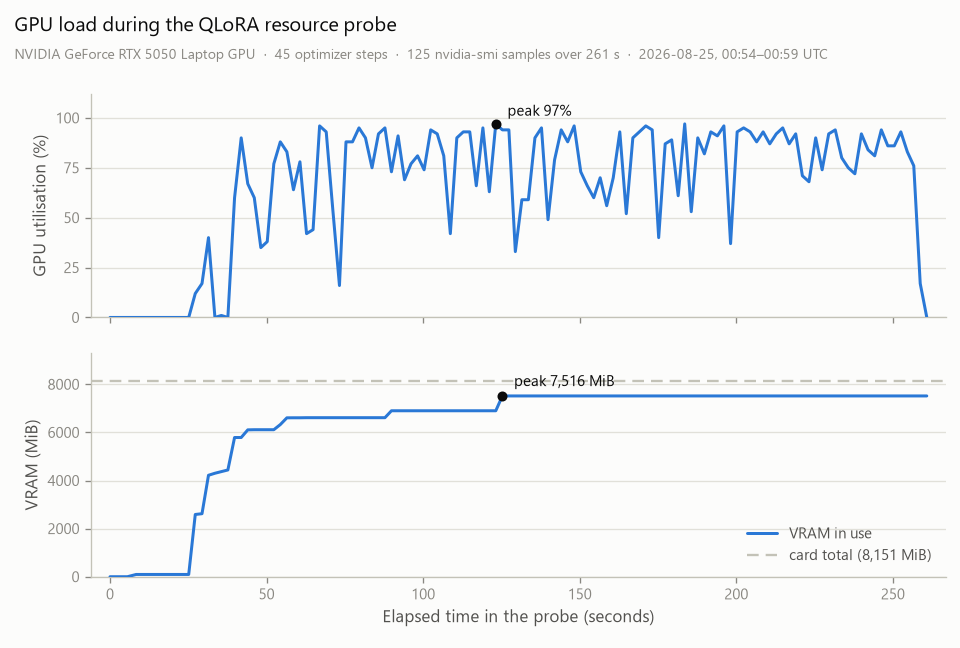
\includegraphics[width=0.92\linewidth]{figures/gpu_telemetry_probe.png}
\caption{GPU usage during the 45-step QLoRA measurement run. Across 125 samples, utilisation peaked at 97 percent and video memory at 7{,}516 of 8{,}151~MiB. This is the short measurement run, not the full training run.}
\label{fig:gpu-telemetry}
\end{figure}

\section{Validation Results}

Both models were trained with the same seed and selected on the same 219 validation messages. Qwen's best checkpoint came at step 200 and PhoBERT's at step 100. Neither produced an unreadable output, and neither called a dangerous message safe.

\begin{figure}[H]
\centering
\begin{tikzpicture}[
  tick/.style={font=\scriptsize, text=black!65},
  val/.style={font=\scriptsize\bfseries, rotate=90, anchor=west}
]
% Truncated vertical scale: y = (score - 0.97) * 180.
\foreach \score/\y in {0.970/0.00,0.980/1.80,0.990/3.60,1.000/5.40} {
  \draw[black!15] (0,\y) -- (7.6,\y);
  \node[tick,anchor=east] at (-0.12,\y) {\score};
}
\draw[black!55] (0,0) -- (0,5.55);
\draw[black!55] (0,0) -- (7.6,0);

\fill[CVBLUE!80] (1.20,0) rectangle (2.00,3.756);
\fill[orange!80] (2.07,0) rectangle (2.87,2.934);
\node[val] at (1.60,3.88) {0.9909};
\node[val] at (2.47,3.06) {0.9863};

\fill[CVBLUE!80] (4.60,0) rectangle (5.40,3.333);
\fill[orange!80] (5.47,0) rectangle (6.27,2.681);
\node[val] at (5.00,3.46) {0.9885};
\node[val] at (5.87,2.81) {0.9849};

\node[font=\small] at (2.04,-0.45) {Accuracy};
\node[font=\small] at (5.44,-0.45) {Macro F1};

\fill[CVBLUE!80] (1.65,6.00) rectangle (2.00,6.25);
\node[font=\small,anchor=west] at (2.12,6.125) {Qwen QLoRA};
\fill[orange!80] (4.65,6.00) rectangle (5.00,6.25);
\node[font=\small,anchor=west] at (5.12,6.125) {PhoBERT};
\end{tikzpicture}
\caption{Fresh validation comparison on the same 219 records. The vertical axis is truncated at 0.970 to show the small differences; one seed provides no variance or significance estimate.}
\label{fig:validation-metric-comparison}
\end{figure}


Figure~\ref{fig:validation-metric-comparison} compares them. Qwen scored higher on both overall measures. PhoBERT was better at recalling bank impersonation, and Qwen was better at recalling Zalo social engineering. Each model was trained and evaluated once, so these numbers justify accepting the selected checkpoints and nothing more.

Speed was left out of this comparison on purpose. The two models produce their answers in completely different ways --- one writes text, the other returns four numbers --- so comparing how long they take would not be measuring the same thing.

\section{Results on the 220 Held-Out Messages}

The 220 held-out messages are the ones neither model saw at any point during training or checkpoint selection. They were set aside when the dataset was first split, and both finished models were run over them exactly once.

Table~\ref{tab:terminal-comparison} gives the results.

\begin{table}[H]
\centering
\renewcommand{\arraystretch}{1.2}
\begin{tabular}{L{3.3cm}rrrrr}
\toprule
\textbf{Model} & \textbf{Accuracy} & \textbf{Macro F1} & \textbf{Weighted F1} & \textbf{Unreadable} & \textbf{Risky called safe} \\
\midrule
Qwen QLoRA & 0.981818 & 0.980493 & 0.981848 & 0 & 1 \\
PhoBERT    & 0.990909 & 0.990892 & 0.990925 & 0 & 1 \\
\bottomrule
\end{tabular}
\caption{Results on the 220 held-out messages. Both models were run once.}
\label{tab:terminal-comparison}
\end{table}

Figure~\ref{fig:terminal-confusion} shows where each model went wrong. Rows are the true label and columns are what the model predicted.

\begin{figure}[H]
\centering
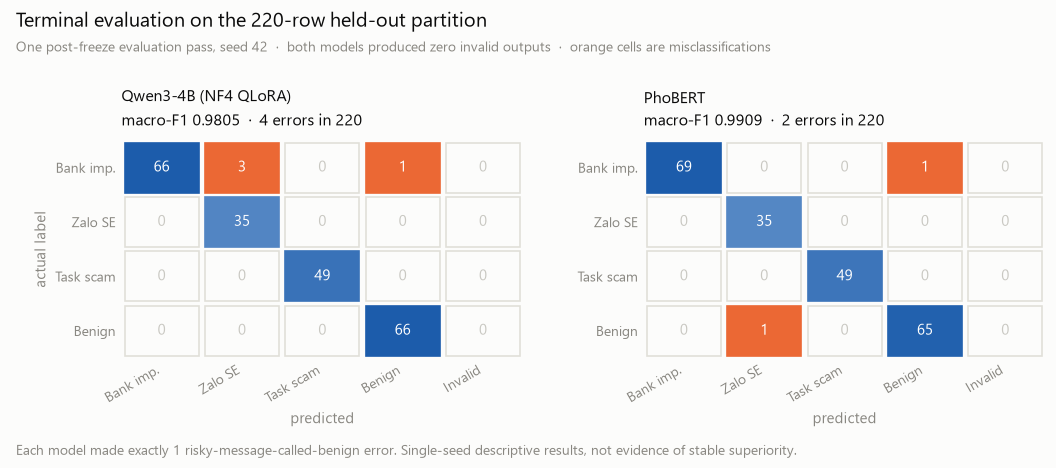
\includegraphics[width=0.98\linewidth]{figures/terminal_evaluation_confusion.png}
\caption{Where each model made mistakes on the 220 held-out messages. Shaded cells off the diagonal are errors: four for Qwen and two for PhoBERT.}
\label{fig:terminal-confusion}
\end{figure}

PhoBERT came out higher on accuracy and on both F1 measures. Qwen came out higher on the benign class, where it raised no false alarms at all while PhoBERT raised one.

The most important column is the last one. A message that is dangerous but gets called safe is the expensive mistake, because the user is told there is nothing to worry about. Both models made exactly one. On the measure that matters most for this system, they tied.

Each model was trained once, so this gap describes what happened in this one run. It is not enough to prove PhoBERT is reliably the better model.

\section{Limits of the Evidence}
\label{sec:evidence-limits}

\begin{enumerate}
\item \textbf{The messages are generated, not collected.} They were written from real public scam warnings rather than taken from real victims. Careful generation, repair, and checking improve the quality of the set, but they cannot show that it matches real scam traffic \cite{kaddour2023synthetic}.

\item \textbf{The manual checking covers a sample.} 100 messages reviewed by hand and 324 labels corrected is real work, but it is not the whole dataset. The 44-out-of-100 pass rate is a warning against reading the judge's high averages as proof that every message sounds natural.

\item \textbf{The judge is not fully independent.} The 296 rewritten Zalo messages were written by a model from the same family as the judge that scored them. For those messages, the judge is checking work related to its own, so its verdict is not a second opinion.

\item \textbf{Everything was run once.} Each model was trained one time with one seed. There is no repeat run to compare against, so there is no way to say how much these numbers would move, and no basis for calling one model reliably better.

\item \textbf{The held-out messages were used once and not reused.} The result was not used to retrain, to repair data, to move a threshold, or to pick a different checkpoint.

\item \textbf{No deployment version was built.} The exported model runs locally, but no version was fitted on all the data afterwards, and no operating threshold was calibrated.

\item \textbf{PhoBERT was not exported to GGUF.} It was kept as a standard Transformers model because it is the comparison baseline rather than the model the system ships, and converting it would not have changed any result reported here.

\item \textbf{Security work is unfinished.} A review of the reorganised code recorded six critical and three warning findings. None of them changes any number in this report, but they do rule out calling the system production-ready.

\item \textbf{Text only.} The system reads pasted text. Screenshots, QR codes, voice calls, and real user traffic are untested.
\end{enumerate}

Within those limits, the project does show a complete chain: a dataset built so that reworded messages cannot leak between splits, hardware measured before committing to a training method, two models trained on the same laptop, training graphs drawn from the run logs, a working exported model, and one evaluation on messages neither model had seen.
